
\documentclass[12pt]{article}
%\documentclass[12pt,twocolumn]{article}

\usepackage{listings}
\usepackage{color}
\usepackage{hyperref}
\usepackage[margin=1.0in]{geometry}
\usepackage{graphicx}

\definecolor{dkgreen}{rgb}{0,0.6,0}
\definecolor{gray}{rgb}{0.5,0.5,0.5}
\definecolor{mauve}{rgb}{0.58,0,0.82}

\lstset{%frame=tb,
  language=bash,
  aboveskip=3mm,
  belowskip=3mm,
  showstringspaces=false,
  columns=flexible,
  basicstyle={\small\ttfamily},
  numbers=none,
  numberstyle=\tiny\color{gray},
  keywordstyle=\color{blue},
  commentstyle=\color{dkgreen},
  stringstyle=\color{mauve},
  breaklines=true,
  tabsize=3, 
  postbreak=\raisebox{0ex}[0ex][0ex]{\ensuremath{\color{red}\hookrightarrow\space}}
}

\begin{document}

\title{Framework for Ice Sheet - Ocean Coupled modelling (FISOC) Manual}
\author{Rupert Gladstone (RupertGladstone1972@gmail.com) \and Lenneke Jong \and Ben Galton-Fenzi}
%\date{Version 0.2, April 2016}
\maketitle

\newpage 
\tableofcontents
\newpage 

\section{Introduction}

The ``Framework for Ice Sheet - Ocean model Coupling" (FISOC) has been written to enable Ice Sheet Models 
(ISMs) and Ocean Models (OMs) to be run as a single executable to address the co-evolution of ice and ocean 
properties.  it is primarily designed to deal with the situation of a floating ice shelf at the interface 
between land ice and open ocean.

In this context an ISM simulates (part of) a marine ice sheet, including both grounded and floating parts, 
representing the dynamic evolution over time of the ice sheet.

An OM simulates the sub-shelf cavity circulation under the floating part of the ice sheet, and optionally also 
a wider ocean domain.

FISOC is a set of code modules and driver built using the Earth System Modelling Framework (ESMF, 
\url{https://www.earthsystemcog.org/projects/esmf/}). 
Some knowledge of the ESMF is essentially in order to fully understand the FISOC code.  It should 
be possible to run FISOC without knowledge of ESMF.

A full description of the physical processes FISOC attempts to simulate are provided in (***
ref GMD paper, not yet written).  
This manual describes how to use FISOC with an ISM and OM for which it has been 
developed (Section~\ref{sec:FISOC_SUG}) and also how to build additional ISM or OM components 
into the FISOC framework (Section~\ref{sec:FISOC_SDG}).

A number of web links are given at various points in this document.  
The links were correct at the time they were added. 
Please contact the authors if any of these are found to be out of date. 




\section{Installing FISOC with established components}
\label{sec:FISOC_install}

FISOC can be obtained by emailing a request to the author.  It is maintained and developed in a 
private GitHub repository.  We intend to make this public late 2016 or early 2017.

FISOC has a simple build process.  The Makefile in the top level FISOC directory contains the 
hard coded dependencies needed to build FISOC code.  The Makefile refers to certain 
environment variables to determine paths and component choices (Section~\ref{sec:EnvVars}). 

Having installed the pre-requisites (Section~\ref{sec:PreReq}), simply run at the command line, 
in the top level FISOC directory:
\begin{lstlisting}
make install
\end{lstlisting}

An example script to build and install FISOC, 'buildFISOCexample.sh', is available in the top 
level FISOC directory.

FISOC has been tested with GNU compilers on Linux Mint using OpenMPI. 



\subsection{FISOC Environment Variables}
\label{sec:EnvVars}

Several environment variables may be used in the build process. 
Some of these are mandatory. 
Variables listed as optional here may be mandatory for configuratons other than 
``dummy''.
These environment variables are not used at run time, only during 
the compilation/installation of FISOC.


\begin{flushleft}
\textbf{ESMFMKFILE}                                \\ 
Required.                                          \\
Tells FISOC where to find key ESMF information.    \\
\vspace{6pt}
\textbf{FISOC\_INSTALL\_DIR}                       \\ 
Optional.                                          \\
Determines where FISOC\_caller will be installed. Defaults to \$HOME/bin. 
The user should also ensure this location is in their \$PATH. \\
\vspace{6pt}
\textbf{FISOC\_MPI}                                \\ 
Optional. Possible value ``yes''.                  \\
Sets preprocessor flag to tell FISOC whether this is a parallel compilation.
Defaults to serial.                                \\
\vspace{6pt}
\textbf{FISOC\_OM}                                 \\ 
Required. Possible values ``dummy'', ``ROMS''.     \\
Determines which OM component will be used.        \\
\vspace{6pt}
\textbf{FISOC\_OM\_INCLUDE}                       \\ 
Optional.                                          \\
Specifies the path where the OM header files are located.\\
\vspace{6pt}
\textbf{FISOC\_OM\_LIBPATH}                       \\
Optional.                                          \\
Specifies the path where the OM library files are located.\\
\vspace{6pt}
\textbf{FISOC\_OM\_LIBS}                          \\
Optional.                                          \\
Specifies the linker directives needed to link the OM library to FISOC. \\
\vspace{6pt}
\textbf{FISOC\_ISM}                                \\
Required. Possible values ``dummy'', ``Elmer''.    \\
Determines which ISM component will be used.       \\
\vspace{6pt}
\textbf{FISOC\_ISM\_INCLUDE}                       \\ 
Optional.                                          \\
Specifies the path where the ISM header files are located.\\
\vspace{6pt}
\textbf{FISOC\_ISM\_LIBPATH}                       \\
Optional.                                          \\
Specifies the path where the ISM library files are located.\\
\vspace{6pt}
\textbf{FISOC\_ISM\_LIBS}                          \\
Optional.                                          \\
Specifies the linker directives needed to link the ISM library to FISOC. \\
\end{flushleft}



\subsection{Pre-requisites}
\label{sec:PreReq}

A Message Passing Interface (MPI) implementation, such as 
OpenMPI is required.\\
 \url{http://www.open-mpi.org/}

The Network Common Data Form (NetCDF) Fortran interface must be available. 
More specifically, NetCDF4 in parallel should be used (this is not the same as PnetCDF). \\
\url{http://www.unidata.ucar.edu/software/netcdf/}

ESMF must be available. ESMF should have been built with NetCDF and MPI 
(see also notes in Appendix~\ref{app:A}). \\
\url{https://www.earthsystemcog.org/projects/esmf/}.

%For example, environment variables like these may be used for the ESMF build
%\begin{lstlisting}
%export ESMF_NETCDF="split"
%export ESMF_NETCDF_INCLUDE="/usr/local/include/"
%export ESMF_COMM="openmpi"
%\end{lstlisting}

Viable ISM and OM components must be available for any physically meaningful simulations
(the build may be tested using ``dummy'' components).  
See Sections~\ref{sec:PreReqElmer} and \ref{sec:PreReqROMS}.


\subsubsection{Elmer/Ice}
\label{sec:PreReqElmer}

***how this should be written depends on whether the FISOC changes to 
Elmer code make it in to the Elmer repository. currently FISOC contains 
top level control structures that replace Elmer ones and the whole of 
Elmer needs to be re-compiled.  We aim to commit these changes to the 
main Elmer/Ice repo.***

***ref and link Elmer/Ice

When compiling FISOC with Elmer/Ice, FISOC needs to know where to 
find the relevant Elmer/Ice libraries.  
This can be done at FISOC compile time through the 
\$FISOC\_ISM
environment variables.  


\begin{lstlisting}
export FISOC_ISM="Elmer"
export FISOC_ISM_INCLUDE="$ELMER_HOME/share/elmersolver/include"
export FISOC_ISM_LIBPATH="$ELMER_HOME/lib/"
export FISOC_ISM_LIBS="-lelmersolver"
\end{lstlisting}





\subsubsection{ROMS}
\label{sec:PreReqROMS}

FISOC has been developed and tested with an ice shelf enabled version of ROMS. 
This is branched from the Rutgers ROMS repository.  Information about the Rutgers ROMS 
can be found at \url{https://www.myroms.org/}.

Development of the ice shelf enabled version  is currently ongoing in a private repository 
(please contact the developers if you need access to this).
A public version of the ice shelf enabled version is also available through github: 
\url{https://github.com/bkgf/romsIceShelf}.  
Please use the "FISOC\_friendly" branch.

***I need to merge the deve version to the public version before releasing this!!!***

Example build scripts can be found in the ROMS/Bin subdirectory of a git clone 
from the repository mentioned above.
It is now assumed that users are familiar with a standard ROMS build process. 

When compiling ROMS for use with FISOC, the following additional environment
variables are needed:
\begin{lstlisting}
export MAKE_SHAREDLIB="Yes"
export LIBDIR="/usr/local/lib"
export MY_CPP_FLAGS=" -DFISOC"
\end{lstlisting}

It is essential to activate the option to compile the ROMS shared library, which 
is done by setting the environment variable MAKE\_SHAREDLIB to any value. 

The shared library will be installed in the location given by the 
 \$LIBDIR environment variable. 

The -DFISOC flag activates preprocessor options.  This includes telling ROMS to use a 
specific hard coded unit rather than outputting to screen.  This relies on the 
same unit being hard coded in the FISOC ROMS wrapper, and results in the ROMS 
messages being sent to file instead of printed to screen.

By default ROMS will install the module files in the directory given by 
 \$SCRATCH\_DIR.  

When compiling FISOC with ROMS, FISOC needs to know where to 
find the relevant ROMS libraries.  
This can be done at FISOC compile time through the 
\$FISOC\_OM
environment variables.  For example:

\begin{lstlisting}
export MY_ROMS_DIR="/home/elmeruser/Source/ROMSIceShelf_devel"
export FISOC_OM="ROMS"
export FISOC_OM_LIBS="-loceanM"
export FISOC_OM_INCLUDE="\${MY_ROMS_DIR}/Build"
export FISOC_OM_LIBPATH="/usr/local/lib"
\end{lstlisting}






%\subsection{Troubleshooting}







\section{Running FISOC}
\label{sec:FISOC_SUG}

The FISOC executable is called FISOC\_caller, and should be located in your path after installation. 
The installation is specific to the choice of component (you need to re-compile if you switch, for 
example, from one ISM to another).  
Beyond choice of components, all run time choices are made in the FISOC\_config.rc file
(Section~\ref{sec:config}), 
or through component specific initialisation.

For example, you can run FISOC in serial like this:
\begin{lstlisting}
FISOC_caller
\end{lstlisting}
You can run FISOC in parallel like this (depending on your system):
\begin{lstlisting}
mpirun -np 4 FISOC_caller
\end{lstlisting}

In the first instance a dummy coupler can be run be setting both environment variables FISOC\_ISM and 
FISOC\_OM to ``dummy'' at compile time.  This can help to test the compilation, and was used during development, 
but performs no meaningful science.  

In verbose mode (Section~\ref{sec:config}) some run time information may be printed to the screen.  
Independently of this, log files are always written, 
with default filenames of ``PET\#.FISOC.Log'', where ``\#'' is a number from 0 upwards indicating the 
``Persistent Execution Thread'' (PET). 
These logs containing run time messages and errors can be helpful with troubleshooting.
Note that FISOC appends to the logs rather than over-writing at run time, so you may wish to delete old logs 
periodically. 

Aside: PET is an ESMF abstraction designed to be general over differing parallel implementations. 
In FISOC, there is always a 1:1 relationship between PETs and MPI processes. 
%(Section~\ref{sec:FISOC_SDG}). 


\subsection{FISOC configuration}
\label{sec:config}

The FISOC config file is named FISOC\_config.rc, and is expected to be present 
in the current directory.  
This is a resource file, as described by the 
ESMF documentation.  It supports different types and also lists. 
In principle, llists of mixed types are supported, though FISOC does not utilise this capability.

FISOC\_config.rc contains code specific to the coupling.  Components may also use their 
independent means for configuration.

Some of the FISOC config entries are required.
This section describes all the valid standard (but note that model-specific non-standard entries 
can be added as required) entries in a FISOC config file as follows:

\begin{flushleft}
\textbf{label:}               [TYPE]   [Required?]                         \\
Description                                                                \\
\vspace{6pt}
\vspace{6pt}
\textbf{ISM\_meshFile:}       [STRING] [optional]                          \\
The name of a netcdf file containing the ISM mesh in ESMF format.          \\
\vspace{6pt}
\textbf{ISM\_configFile:}     [STRING] [optional]                          \\
The name of the ISM-specific config file.                                  \\
\vspace{6pt}
\textbf{FISOC\_ISM\_ReqVars:} [STRING] [required]                          \\
List of variable names required to be provided by the ISM.                 \\
\vspace{6pt}
\textbf{FISOC\_ISM\_DerVars:} [STRING] [required]                          \\
List of variables derived by FISOC from the ISM vars.                      \\ 
To be calculated from ISM vars by hard coded routines in FISOC\_ISM.       \\
\vspace{6pt}
\textbf{ISM2OM\_vars:}        [STRING] [required***(default all?)]                          \\
List of variables to be passed from the ISM to the OM.                     \\ 
\vspace{6pt}
\textbf{ISM\_grdType:}        [STRING] [required]                          \\
Which ESMF object to use.  Valid values are ESMF\_mesh and ESMF\_grid.     \\
\vspace{6pt}
\vspace{6pt}
\vspace{6pt}

\textbf{OM\_configFile:}      [STRING] [optional]                          \\
The name of the ISM-specific config file.                                  \\
\vspace{6pt}
\textbf{FISOC\_OM\_ReqVars:}  [STRING] [required]                          \\
List of variable names required to be provided by the OM.                  \\
\vspace{6pt}
\textbf{OM\_ReqVars\_stagger:} [STRING] [optional]                         \\
Corresponding exactly to the above, descriptions of the grid stagger for each var. \\
\vspace{6pt}
\textbf{FISOC\_OM\_DerVars:}  [STRING] [required]                          \\
List of variables derived by FISOC from the OM vars.  
To be calculated from ISM vars by hard coded routines in FISOC\_OM.        \\
\vspace{6pt}
\textbf{OM\_writeNetcdf:}   [LOGICAL] [optional]                           \\
Switch for dumping the OM import and export variables to NetCDF files.
Defaults to .TRUE.                                                         \\
\vspace{6pt}
\textbf{output\_dir:}  [STRING] [optional]                                 \\
Path to directory (must already exist) to which to write the NetCDF files. 
Defaults to current directory.                                             \\
\vspace{6pt}
\textbf{OM\_initCavityFromISM:}  [LOGICAL] [optional]                      \\
Switch to allow the OM to overwrite its cavity geometry with ISM\_z\_l0 
during the second phase of initialisation.
Defaults to .FALSE.                                                        \\
\vspace{6pt}
\textbf{OM2ISM\_vars:}        [STRING] [required***(default all?)]                          \\
List of variables to be passed from the OM to the ISM.                     \\ 
\vspace{6pt}
\textbf{OM\_grdType:}        [STRING] [required]                           \\
Which ESMF object to use.  Valid values are ESMF\_mesh and ESMF\_grid.     \\
\vspace{6pt}
\textbf{OM\_cavityUpdate:}   [STRING] [optional]                           \\
How to process ISM ice draft for use in OM.  Valid values are RecentIce    \\
(default), Rate, CorrectedRate, and Linterp.                               \\
\vspace{6pt}
\vspace{6pt}

\textbf{OM\_outputInterval:} [INTEGER][optional]                           \\
FISOC collects OM output once every OM\_outputInterval OM timesteps. 
Defaults to 1.  dt\_ratio/OM\_outputInterval must be integer.              \\
\vspace{6pt}
\textbf{OM\_dt\_sec:}         [INTEGER][required]                          \\
OM timestep length in seconds.                                             \\
\vspace{6pt}
\textbf{dt\_ratio:}          [INTEGER][required]                           \\
ISM/OM timestep ratio.                                                     \\
\vspace{6pt}
\textbf{start\_year:}        [INTEGER][required]                           \\
Start year and month define the start time of the coupled simulation.      \\
\vspace{6pt}
\textbf{start\_month:}       [INTEGER][required]                           \\
\vspace{6pt}
\textbf{end\_year:}          [INTEGER][required]                           \\
End year and month define the finish time of the coupled simulation.       \\
\vspace{6pt}
\textbf{end\_month:}         [INTEGER][required]                           \\
\vspace{6pt}
\vspace{6pt}

\textbf{verbose\_coupling:}  [LOGICAL][required]                           \\
If true, some run time information is printed to the screen.  A log file is always 
written, but writing to the log during timestepping is suppressed when 
verbose\_coupling is false.\\
\end{flushleft}



\subsubsection{FISOC variables}
\label{sec:FISOCvars}

The union of \textbf{FISOC\_ISM\_ReqVars}, \textbf{FISOC\_ISM\_DerVars}, \textbf{FISOC\_OM\_ReqVars} 
and \textbf{FISOC\_OM\_DerVars} describes the full set of variables required by FISOC for a given simulation. 
Valid values are given in Table~\ref{tab:vars}.
Note that the units given in Table~\ref{tab:vars} are suggested units.  FISOC doesn't care about units, but 
the user must ensure unit consistency.  There may be hard coded unit assumptions in the model specific 
wrappers.

***variable names: sort out dddt and dBdt\_l0.  consistent naming convention needed.

\begin{table}
  \begin{center}
    \begin{tabular}{ l|l|l }
      Variable              & Description                                  & Units \\
      \hline
      ISM\_temperature\_l0  & Ice temperature at the ice ocean interface.  & K \\
      ISM\_temperature\_l1  & Ice temperature in the ISM one level above   & K \\
                            & the ice ocean interface.                     &   \\ 
      ISM\_z\_l0            & Height relative to sea level of the ice      & m \\
                            & base.                                        &   \\
      ISM\_z\_l1            & Height relative to sea level of the first    &   \\
                            & ISM model level above the ice base.          & m \\
      ISM\_z\_l0\_previous  & Height relative to sea level of the ice      &   \\
                            & base one timestep previously.                & m \\
      ISM\_dTdz\_l0         & Vertical temperature gradient in the ice     &   \\
                            & at the ice base.                             & K/m \\
      ISM\_dddt             & Rate of change of the height of the ice      &   \\
                            & base relative to sea level with respect to   &   \\
                            & time.                                        & m/a \\
      ISM\_velocity\_l0     & Ice flow velocity at the ice base            & m/a \\
      OM\_dBdt\_l0          & Ice shelf basal melt rate                    & m/a \\
      OM\_temperature\_l0   & Ocean temperature at the ice ocean           &   \\
                            & interface  ***or is this the ocean model...  &   \\
                            & guessing the ice temperature at the interface&   \\
    \end{tabular}
  \end{center}
  \caption{FISOC standard variables and typical units.  
    Note that heights relative to sea level are always positive upward.}
  \label{tab:vars}
\end{table}

As a naming convention, ``z'' refers to the vertical coordinate, and ``l0'' and ``l1'' refer to the 
model level at the ice-ocean interface (this would typically be the lowest level of the ISM or 
the uppermost level of the OM) and one level above it, respectively.

FISOC outputting occurs on the ocean grid, and consists of dumping both the import and 
export fields to netcdf files. 
\textbf{FISOC\_ISM\_ReqVars} may contain variables that are required only so that they can be written 
out on the ocean grid (typically as a sanity check) rather than actuallly being needed by the OM.


The list of derived variables, \textbf{FISOC\_ISM\_DerVars}, indicates which variables are needed by the 
OM but are not calculated by the ISM or its wrapper. 
The methods for calculating the derived variables are hard coded in FISOC\_ISM.f90. 
Valid values for  \textbf{FISOC\_ISM\_DerVars} include:

ISM\_z\_l0\_previous.  This is the depth of ice base at previous ISM timestep. This is simply stored 
in memory.  No calculation is required, but this variable is needed for the other ``derived'' variables. 

ISM\_dTdz\_l0.  Temperature gradient at ice base.  This is calculated as 
\begin{equation}
ISM\_dTdz\_l0 = \frac{ISM\_temperature\_l1 - ISM\_temperature\_l0}{ISM\_z\_l1 - ISM\_z\_l0}
\end{equation}

ISM\_dddt.  Rate of change of depth of ice base.  This is calculated as 
\begin{equation}
ISM\_dddt = \frac{ISM\_z\_l0 - ISM\_z\_l0\_previous}{ISM\_dt}
\end{equation}

Not all ISM variables need to be passed to the OM, and vice versa.  
This choice is made by the 
user through use of configuration options ISM2OM\_vars and OM2ISM\_vars.  
These options alow the user to specify a subset of the full set of 
required and derived variables that will be passed to the other component 
in a given simulation.  An empty list can be used to avoid any variables 
being passed between components.  This can be useful during testing and 
troubleshooting.

A note on efficiency: All the ISM and OM variables are regridded and passed 
to the wrapper for the opposite component.  It is at the model-specific 
wrapper level that ISM2OM\_vars and OM2ISM\_vars are checked.  If regridding 
becomes a significant proportion of FISOC's computational cost this 
should be re-implemented to reducenon-essential regridding operations.





\subsubsection{Updating the ice shelf cavity for the OM}

See the FISOC GMD paper (***ref) for more details about updating the ocean 
representation of the ice shelf cavity. 
Several options are available through FISOC, from the simplest option of using 
the most recent cavity geometry from the ISM to update the OM representation of 
cavity geometry to smoother options via either interpolation in time or specifying 
a rate of change of cavity geometry.

The options (summarised in Table~\ref{tab:cavity}) are all implemented within FISOC, 
based on the cavity geometry 
calculated by the ISM.  Some options are through FISOC derived variables, as described 
in Section~\ref{sec:FISOCvars}.  The key ISM output from which all cavity options 
are calculated is ISM\_z\_l0.  

\begin{table}
  \begin{center}
    \begin{tabular}{ llll }
      Cavity option  & Summary                                    & Required ISM2OM \\
                     &                                            &  variable       \\
      \hline
      RecentIce      & Most recent ice draft from ISM             & ISM\_z\_l0      \\
      Rate           & Rate of change of ice draft from two most  & ISM\_dddt       \\
                     & recent ISM steps                           &                 \\
      CorrectedRate  & As above with additional drift correction  & ISM\_dddt       \\
      Linterp        & Time-interpolated ice draft from two most  & ISM\_z\_l0\_linterp \\
                     &  recent ISM steps                          &                  \\
    \end{tabular}
  \end{center}
  \caption{
    Cavity update options.  Note that of the possible ISM cavity variables 
    (ISM\_z\_l0, ISM\_z\_l0\_linterp, ISM\_dddt) only the required variable 
    (third column) should be passed to the OM (constrained using ISM2OM\_vars).
  }
  \label{tab:cavity}
\end{table}





\subsubsection{Grids and meshes}
OM\_grdType and ISM\_grdType refer to the type of ESMF object to be used for holding information about 
the model grid.  Typically models utilising unstructured meshes (e.g. Elmer/Ice) would use an 
ESMF\_mesh object for holding mesh information in FISOC and models utilising structured grids 
(e.g. ROMS) would use an ESMF\_grid object for holding grid information in FISOC.








\subsection{Timestepping}
Asynchronous timestepping.
***fill in this section we've implemented both tight coupling (ice and ocean both running 
on the same timescale) and loose coupling (for longer time scales where the ocean is run 
to steady state then the ice sheet continues until significant change has occurred in the cavity).


\subsection{Running FISOC with Elmer/Ice} 
For dynamic linked libraries, shared object files may be needed at run time.  
This can be ensured through use of 
the \$LD\_LIBRARY\_PATH environment variable. 

For example (it is assumed \$ELMER\_HOME was set during Elmer installation):
\begin{lstlisting}
export LD_LIBRARY_PATH="$FISOC_ISM_LIBPATH/:$LD_LIBRARY_PATH"
\end{lstlisting}

As with a normal Elmer/Ice simulation, the mesh should be partitioned into the 
same number of partitions as the number of processors (which is the same as the number of 
ESMF PETs and DEs, but don't worry if you don't know what those things are). 

More information about Elmer, and especially Elmer/Ice, can be found on several sources 
on the internet.

\begin{flushleft}
\url{https://www.csc.fi/web/elmer}\\
\url{http://www.nic.funet.fi/pub/sci/physics/elmer/doc/}\\
\url{http://elmerice.elmerfem.org/}\\
\url{http://elmerice.elmerfem.org/wiki/doku.php}\\
\url{http://www.elmerfem.org/forum/}\\
\end{flushleft}



\subsubsection{Elmer/Ice specific configuration}

The following options in the FISOC configuration file are used by Elmer/Ice.  These 
are non-standard configuration options.

\begin{flushleft}
\textbf{ISM\_BodyID:} [INTEGER] [required]                               \\
The body ID of the surface on which interactions with the ocean occurs.  
Typically this will be the lower surface, defined as a boundary in the   
Elmer/Ice mesh file and as a body in the boundary condition section of   
the .sif.                                                                \\
\vspace{6pt}
\textbf{ISM\_ProjVector:} [INTEGER LIST] [optional]                      \\
3D vector describing the view direction for use in node ordering of      
elements.  Default down.  NYI                                            \\
\vspace{6pt}
\end{flushleft}





\subsection{Running FISOC with ROMS}
\label{sec:runningROMS}

FISOC needs to access the shared library at run time.  One way of ensuring this 
is to add the location of the library to the \$ LD\_LIBRARY\_PATH variable, e.g.:
\begin{lstlisting}
export LD_LIBRARY_PATH="$FISOC_OM_LIBPATH/:$LD_LIBRARY_PATH"
\end{lstlisting}

ROMS writes a lot of information to the screen when run alone.  
When run through FISOC this is redirected to a text file. 
The file name is given by \textbf{OM\_stdoutFile}, 
which must be provided in the FISOC config file 
whenever ROMS is used.

The number of processes to launch FISOC with must be consistent with the number of 
partitions in the ROMS grid.  This is set in the \textbf{OM\_configFile} by the 
Ntile parameters.  For example, the following gives 4 partitions
\begin{lstlisting}
      NtileI == 1                               ! I-direction partition
      NtileJ == 4                               ! J-direction partition
\end{lstlisting}
%This could be launched with
%\begin{lstlisting}
%mpirun -np 4 FISOC_caller
%\end{lstlisting}

Some of the ROMS configuration information is in a .dat file.
The name of this file is given in the ROMS configuration file, the .in file.
When running ROMS through FISOC, the full path of the .dat file must be 
given in the .in file.

\subsubsection{ROMS preprocessor directives}
Some aspects of the ROMS configuration are controlled through preprocessor directives.  
ROMS must be recompiled if these are changed.  
For example, there is a file located somewhere like 
\begin{lstlisting}
ROMS/Include/iceshelf2d.h
\end{lstlisting}
This file contains statements like this:
\begin{lstlisting}
#define ICESHELF
#ifdef ICESHELF
# undef ICESHELF_2EQN_VBC
# define ICESHELF_3EQN_VBC
# undef ICESHELF_TEOS10
# undef ICESHELF_MORPH
# define LIMIT_ICESTRESS
#endif
\end{lstlisting}
In some cases changes are needed to be made to FISOC corresponding with these settings. 
These are made to the hard coded values of variables defined at the head of the ROMS 
wrapper module, contained in the file FISOC\_OM\_Wrapper\_ROMS.F90, with the 
parameter  attribute. 
Currently the following are in use, and further additions may be made as required.
\begin{lstlisting}                                                                                           
  LOGICAL, PARAMETER :: ROMS_MASKING = .FALSE.
  LOGICAL, PARAMETER :: ROMS_SPHERICAL = .FALSE.
\end{lstlisting}
If these values need to be changed FISOC will of course need to be compiled again.





\subsection{Troubleshooting}

If the error messages to the screen are not helpful, remember to check whether useful 
information has been logged.  By default this will be in files in the current directory 
with names like PETX.FISOC.Log (where X is a process number).

A segmentation fault has been known to occurr in the case of an incorrect path to the ROMS 
configuration file (the .in file). 

Note that DMUMPS error codes, should they occur, can be found in the MUMPS user guide.
MUMPS is often used by Elmer/Ice.
http://mumps.enseeiht.fr/doc/userguide\_5.0.1.pdf

Errors like the following can ocurr (in the log files) when the number of processes is 
not consistent with the number of component partitons (this example involves ROMS):
\begin{lstlisting}
20151119 112603.491 ERROR            PET0 ESMCI_DistGrid.C:1200 ESMCI::DistGrid::create() Value unrecognized or out of range - deBlockList contains out-of-bounds elements
20151119 112603.491 ERROR            PET0 ESMCI_DistGrid_F.C:152 c_esmc_distgridcreatedb() Value unrecognized or out of range Internal subroutine call returned Error
20151119 112603.491 ERROR            PET0 ESMF_DistGrid.F90:1220 ESMF_DistGridCreateDB() Value unrecognized or out of range - Internal subroutine call returned Error
20151119 112603.491 ERROR            PET0 src/FISOC_OM_Wrapper_ROMS.f90:612 Value unrecognized or out of range - Passing error in return code
20151119 112603.491 ERROR            PET0 src/FISOC_OM_Wrapper_ROMS.f90:120 Value unrecognized or out of range - Passing error in return code
\end{lstlisting}

Errors like the following can occur if a component wrapper attempts to access a field 
that has not been created by FISOC, i.e. a field that is not in the list of
required variables in the FISOC config file (Section~\ref{sec:config}) 
(this example involves FISh):
\begin{lstlisting}
20151207 152613.483 ERROR            PET0 ESMCI_Container_F.C:165 ESMCI::Container::get() Invalid argument key does not exist
20151207 152613.484 ERROR            PET0 ESMCI_Container_F.C:448 c_esmc_containergetfield() Invalid argument Internal subroutine call returned Error
20151207 152613.484 ERROR            PET0 ESMF_Container.F90:589 ESMF_ContainerGetField() Invalid argument - Internal subroutine call returned Error
20151207 152613.484 ERROR            PET0 ESMF_FieldBundle.F90:1456 ESMF_FieldBundleGetItem() Invalid argument - Internal subroutine call returned Error
20151207 152613.484 ERROR            PET0 src/FISOC_ISM_Wrapper_FISh.f90:198 Invalid argument - Passing error in return code
\end{lstlisting}



\section{Post processing}

It is expected that the OM and ISM components will output data in their usual formats, 
and that this will form the basis for most output visualisation and post-processing.
FISOC does however have the capcity to output both ISM and OM fields on the OM grid 
in netcdf format.

Scripts for visualising these outputs may be developed at some point, but no firm 
plans exist.  If/when developed, they will be located in the FISOC\_pp directory.
There is currently an inflexible script and unfriendly script used as a sanity 
check during development.

The script requires a recent python installation and the netcdf4-python module.




\subsection{Netcdf4-python installation notes}

Depending on your python installation, you may need to run something like this
before installing netcdf4-python:
\begin{lstlisting}
sudo apt-get install python-dev
\end{lstlisting}
More information about the netcdf4-python module can be found here:\\
\url{http://unidata.github.io/netcdf4-python/}\\
\\
You can clone or download the latest netcdf4-python code from the GitHub 
repository:
\begin{lstlisting}
git clone git@github.com:Unidata/netcdf4-python.git 
\end{lstlisting}
Then build and install the netcdf4-python library like this:
\begin{lstlisting}
python setup.py build
python setup.py install
\end{lstlisting}
Install may require root privileges.
You may need to restart your shell.  

A minor discrepancy between the python setup script and the way nc-config 
retrieves relevant flags may lead to errors if mpi wrappers are used. 
This issue should probably be considered a bug in nc-config. 
More information (and a dirty fix) can be found here:\\
\url{https://github.com/Unidata/netcdf4-python/issues/491}\\






\section{FISOC development and incorporating new components}
\label{sec:FISOC_SDG}

FISOC is designed such that the only code developments for new components should be the creation 
of model-specific wrappers: FISOC\_OM\_Wrapper\_XXX.f90 or FISOC\_ISM\_Wrapper\_XXX.f90, where 
XXX should be replaced by the component's name.

Any new OM or ISM component to be used with FISOC must first be ESMF compliant.  This basically 
means that it should have an initialise, run and finalise routine, and that the developer can 
provide the component's grid and variables in ESMF compatible formats through the new wrapper.
The ESMF web site provides furtehr documentation.
https://www.earthsystemcog.org/projects/esmf/

If it is found that changes to other aspects of the FISOC code are required, this should be 
implemented in collaboration with the FISOC core developers.

If you write a new model-specific wrapper you are encouraged to submit it to the FISOC repository.
Please contact the FISOC developers or submit a pull request through github.

The FISOC code structures are summarised in Figure~\ref{fig:codeStruct}.
 
***update the picture

***add description here or perhaps self evident?

***add section on getting help with FISOC? emphasize try component on its own first.  dont ask FISOC devs if the problem is entirely in one component.

\begin{figure}[t]
  \vspace*{2mm}
  \begin{center}
    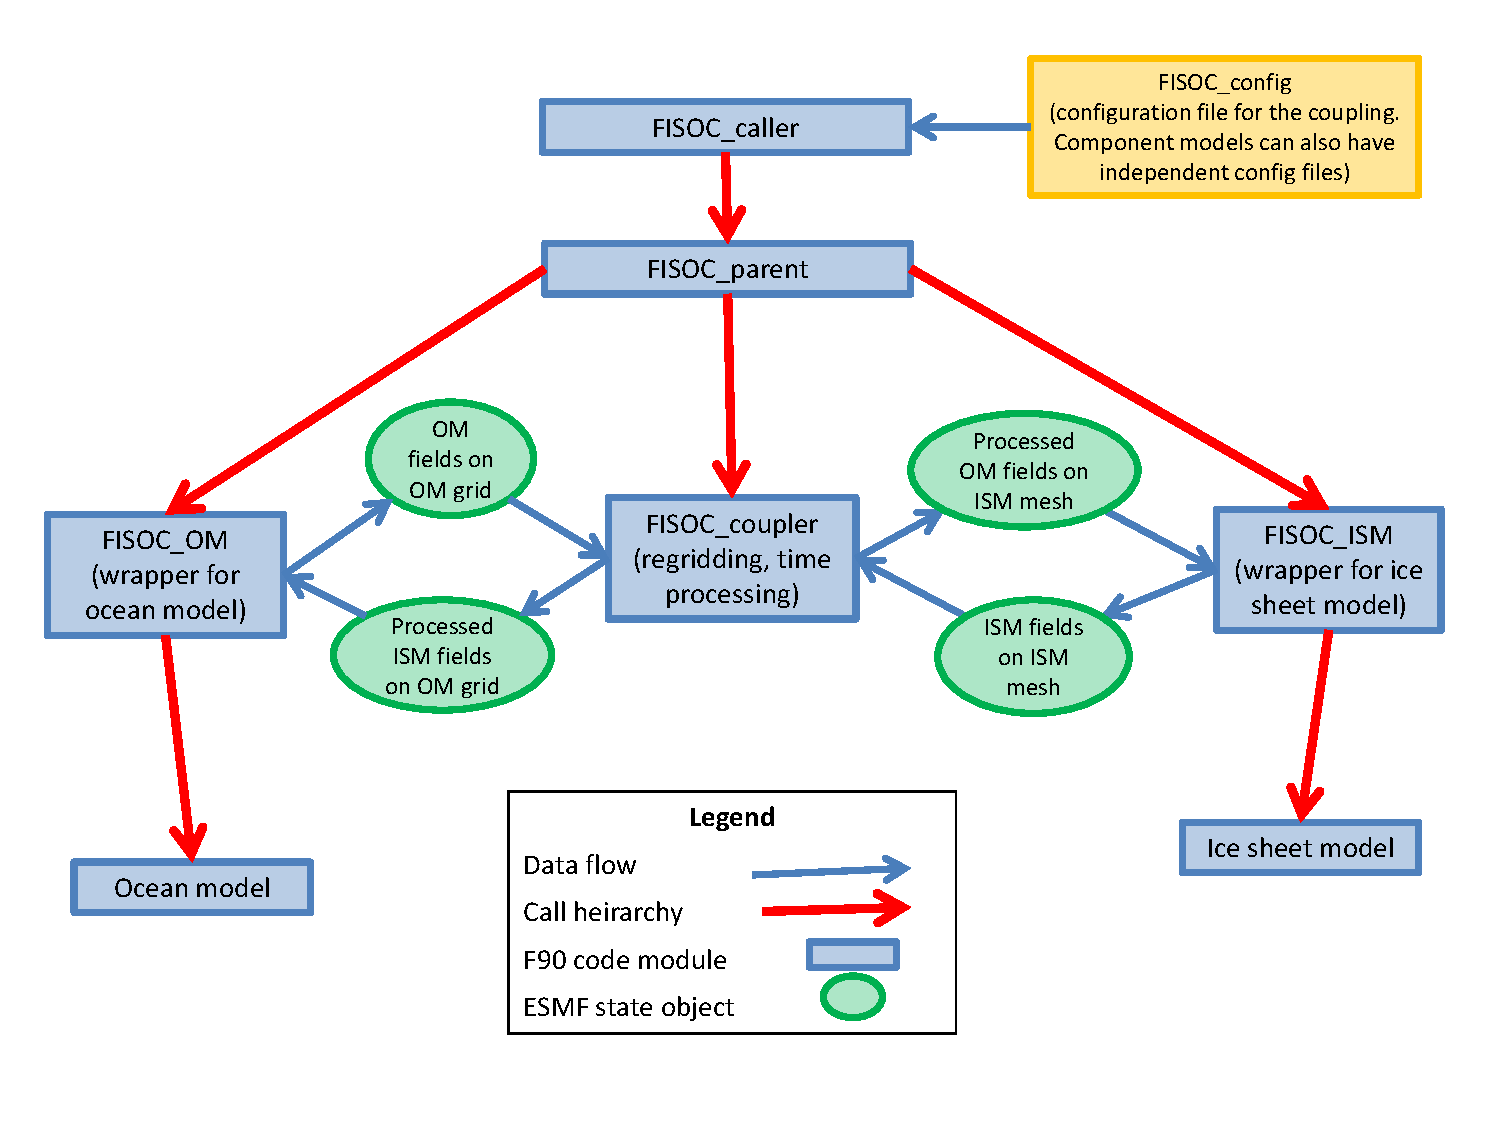
\includegraphics[width=17cm]{FISOC_structure.pdf}
  \end{center}
  \caption{FISOC code and data structures.}
  \label{fig:codeStruct}
\end{figure}


\subsection{Coding practices}

A new component wrapper  should be in a Fortran 90 module.  
All modules should contain the ``implicit none'' statement at the top (immediately after any 
``USE'' statements).  This property will be inherited by all procedures in the module.

FISOC modules have the private attribute, with only required procedures being 
made public. 
New model-specific wrapper modules should ensure that the initialise, run and finalise 
subroutines are public. 

When writing new wrapper modules, the existing wrapper modules may be used as a template, 
providing examples of the required interfaces.
Once the FISOC code base stabilises we may provide a full description of the required interface 
here, but for now adapting an existing wrapper module is advised.


\subsubsection{Error handling}

ESMF provides defensive error handling, with error codes and error messages passed up the 
call stack. 
FISOC implements ``fail-fast'' error handling, with errors generally being considered 
fatal. 
Exceptions to this may be made where it is safe to do so (e.g. where a default value can be 
used in the event of  failure to find a config parameter).
All calls to ESMF routines have return codes checked immediately, and errors logged.
If components (OM or ISM) provide a return code or error code, 
this should be checked by the component wrapper.

Note that many FISOC subroutines contain a return code, but these are mostly not used in 
practice.  Since errors are generally considered instantly fatal in FISOC, execution will 
generaly not get as far as returning a failure code. 
If a more defensive rather than fail-fast approach is adopted in the future these return 
codes can be used.



\subsection{Configuration options}

The configuration file must be called ``FISOC\_config.rc'' and is compatible with ESMF 
config methods.  
An ESMF\_config object is automatically created from this file.

There may be some parameters that are derived from config parameters.  
The FISOC\_utils module provides subroutines under the 
FISOC\_ConfigDerivedAttribute interface 
for obtaining derived config parameters.
These subroutines can be viewed informally as additional methods to complement the ESMF config access methods. 

An advantage of the way the config object is used is that new config arguments can be added and 
used in the coupling without requiring developments to any code other than the new wrapper. 
The config object can be passed to the wrapper and accessed directly. 


%\subsection{ISM wrapper}

%\subsection{OM wrapper}

%\section{Future developments}



\clearpage

\appendix

\section{Pre-requisite installation notes}
\label{app:A}
The following commands worked to install NetCDF and ESMF on a Linux Mint system in 2015.
Some pre-requisites for netcdf were also installed.
The system already had a working OpenMPI installation.



\begin{lstlisting}[language=bash]


# instructions on installing ESMF can be found here:
# http://www.earthsystemmodeling.org/esmf_releases/last_built/ESMF_usrdoc/node9.html

# netcdf instructions
# http://www.unidata.ucar.edu/software/netcdf/docs/netcdf-install.html

cd /somewhere/to/download/and/compile/source/code

sudo apt-get install m4

wget ftp://ftp.unidata.ucar.edu/pub/netcdf/netcdf-4/zlib-1.2.8.tar.gz
tar -xzf zlib-1.2.8.tar.gz 
cd zlib-1.2.8
 ./configure --prefix=/usr/local/
 make check
 sudo -E make install
cd ..

wget ftp://ftp.unidata.ucar.edu/pub/netcdf/netcdf-4/hdf5-1.8.13.tar.gz	
tar -xzf hdf5-1.8.13.tar.gz 
cd hdf5-1.8.13
 # Note the O0 flag in the next line.  The default is O3, 
 # which is strong optimisation.  This can result in failed 
 # checks on some systems.
 CFLAGS="-O0 -fPIC" CC=mpicc CXX=mpiCC FC=mpif90 ./configure --prefix=/usr/local/ --with-zlib=/usr/local  --enable-fortran --enable-parallel --enable-shared
 make check
 sudo -E make install
cd ..

# note that netcdf fortran library is now compiled from a 
# seperate source from the main netcdf c library. Install 
# the c library first, and make sure to create the shared
# object file. 
wget ftp://ftp.unidata.ucar.edu/pub/netcdf/netcdf-4.3.3.tar.gz
tar -xzf netcdf-4.3.3.tar.gz 
cd netcdf-4.3.3/
 LIBS=-ldl CC=mpicc CXX=mpiCC FC=mpif90 CPPFLAGS=-I/usr/local/include/ LDFLAGS=-L/usr/local/lib/  ./configure --prefix=/usr/local --enable-parallel 
 make check
 sudo -E make install
cd ..

wget ftp://ftp.unidata.ucar.edu/pub/netcdf/netcdf-fortran-4.4.2.tar.gz
tar -xzf netcdf-fortran-4.4.2.tar.gz 
cd netcdf-fortran-4.4.2
 LIBS=-ldl CC=mpicc CXX=mpiCC FC=mpif90 LDFLAGS=-L/usr/local/lib/ CPPFLAGS="-I/usr/local/include -DUSE_NETCDF4"  ./configure --prefix=/usr/local
 make check
 sudo -E make install
cd ..

# convenient viewer for contents of netcdf files (not essential)
sudo apt-get install ncview

# ESMF requires ESMF_DIR and probably other environment variables.  
# These can be set at the command line or, for example, in your 
# .bashrc file.  These might work:
export ESMF_DIR="/top/level/directory/for/esmf/"
export ESMF_NETCDF="split"
export ESMF_NETCDF_INCLUDE="/usr/local/include"
export ESMF_NETCDF_LIBPATH="/usr/local/lib"
export ESMF_COMM="openmpi"
export ESMF_PIO="internal"
                                                                                                              
wget downloads.sourceforge.net/project/esmf/ESMF_6_3_0r/ESMF_6_3_0rp1/esmf_6_3_0rp1_src.tar.gz
tar -xf esmf_6_3_0rp1_src.tar.gz
cd esmf 
 make check
 sudo -E make install
cd ..

# In order to actually use ESMF you must set the environment 
# variable ESMFMKFILE.  If you didn't use environment 
# variables to specify the install location this make file 
# will probably end up somewhere like this:
export ESMFMKFILE="$ESMF_DIR/DEFAULTINSTALLDIR/lib/libO/Linux.gfortran.64.openmpi.default/esmf.mk"


\end{lstlisting}

\end{document}
